%%% -*- coding: utf-8 -*-
\newpage

\chapter{Related Work}
\label{chap:related}

In this chapter, we make a brief review of the works related to ours. Section \ref{sec:spatiotemporal} contains work related to the core method of this work. The next three sections describe work related to the applications we propose based on our core method.

\section{Spatiotemporal Localization of Actors}
\label{sec:spatiotemporal}


The task of detecting and tracking actors in videos has been the focus of much research. In early 2004, Küblbeck and Ernst \cite{facetracking_2} used an illumination invariant approach for face detection combined with a tracking mechanism performed by means of continuous detections. Kim \emph{et al.} \cite{face_tracking} addressed the problem of tracking faces in noisy videos using a tracker that adaptively builds a target model reflecting changes in appearance, typical of a video setting. This kind of approach does not perform well in the task of spatiotemporal localization of actors because they can only track them when they are continuously present on the video. Differently, the approach we use, which is based on clustering, does not require the actors to be continuously present on the video.

More similar to ours, recent works have investigated the use of clustering for grouping faces of actors in video and, consequently, providing the spatiotemporal localization of them. Tapaswi \emph{et al.} \cite{video_face_clustering} propose Ball Cluster Learning~(BCL), a supervised approach to carve the embedding space into balls of equal size, one for each cluster. The radius of such ball is translated to a stopping criterion for iterative merging algorithms. Sharma \emph{et al.} \cite{self_supervised} propose a self-supervised Siamese network for video face clustering that can also be used in scenarios where tracks of actors are not available, such as image collections. The approach we use can also be applied to image collections, as further explained in Section \ref{chap:face_recognition}, but it differs in the sense that we use pre-trained CNNs (Convolutional Neural Networks) and traditional clustering algorithms for performing this task. 

It is worth mentioning that, in this dissertation, we do not intend to directly compare or propose a better method for the task of spatiotemporal localization of actors than the existing ones. Instead, we intend to investigate to what extent our method opens up novel approaches for the three chosen applications and the benefits that can be achieved with our approach.

\section{Video Face Recognition}
\label{sec:video_face}

Many methodologies have been proposed for \emph{Video Face Recognition}, most commonly relying on comparing selected facial features of a given image with features of faces within a database.
Using only one sample reference image of a person's face for the comparison may result in classification errors due to factors related to variations in lighting, image resolution, angle, etc.~\cite{598229}.
To overcome this problem, some face recognition approaches use multiple face samples for comparison. However, this strategy does not scale well as the complexity is a function of the number of samples.
Other approaches treat the face recognition task as a classification problem~\cite{dadi2016improved, ghosal}, where a classifier model learns rules to assign faces to previously known classes within a dataset, where each class corresponds to one person.
Nonetheless, this kind of approach does not deal well when new classes are incorporated because of the need to retrain the classification models.
Moreover, when dealing with video, these kinds of methods have to be applied to each frame, again increasing their complexity.


Traditional deep learning models for face recognition such as DeepFace~\cite{taigman2014deepface} and DeepID~\cite{sun2014deep} use a CNN with fully connected layer output to produce a representation of high-level features (face embeddings) from an input image, followed by a softmax layer to indicate the identity of classes. Other approaches, such as FaceNet~\cite{schroff2015facenet}, can directly measure the similarity among faces using euclidean space. Inspired by DeepID, this model uses the \textit{triplet loss} as the loss function to estimate similarity to one character's face to a  collection of other faces. Triplet loss improves the accuracy of the  CNN output by minimizing the euclidean distance between the anchor and the positive (face of the same identity) while maximizing the distance between the anchor and the negative (face of another identity). In this work, we evaluated different pre-trained CNN backbones on VGGFace2 dataset~\cite{cao2018vggface2} to generate the face embeddings. 

Proprietary systems for face recognition and matching are widely used by social network platforms. For instance, Facer~\cite{hazelwood2018applied} is Facebook's face detection and recognition framework. Given a photograph, it first detects all the faces. Then, it runs a  deep model to determine the likelihood of that face belonging to one of the top-N user friends. This allows  Facebook to suggest which friends the user might want to tag within the uploaded photographs. FindFace\footnote{https://findface.br.aptoide.com/app} is an app that matches photos to profile pictures on VKontakte,\footnote{https://vk.com/} a Russian social networking website similar to Facebook. FindFace uses a deep model developed by NTech Lab that won the \textit{2017 IARPA Face Recognition Prize Challenge} (FRPC)~\cite{grother20172017}  in two nominations out of three (“Identification Speed” and “Verification Accuracy”). Similarly, our method can detect faces in videos and automatically recognize their identities by a clustering-based algorithm that uses a knowledge base with the faces pre-identified as a reference; however, a comparison with such methods was not possible due to access restrictions.

Some recent works are focused on video face recognition. Pena \emph{et al.} \cite{globofacestream} proposed a face recognition system to detect characters within videos, called~\textit{Globo Face Stream}. Their method uses a Histogram of Oriented Gradients (HOG) feature combined with a linear classifier to detect faces. Next, they use  FaceNet to generate the embeddings, followed by the euclidean distance calculus to measure the similarity among faces. Yang \emph{et al.} \cite{yang2017neural} proposed a deep network for video face recognition called NAN (Neural Aggregation Network). They use a CNN to generate the embeddings, followed by an aggregation module that consists of two attention blocks that adaptively aggregate the feature vectors to form a single feature inside the convex hull spanned by them. Rao \emph{et al.} \cite{rao2017attention} proposed a method for video face recognition based on attention-aware deep reinforcement learning. They formulated the process of finding the attention of videos as a Markov decision process and training the attention model without using extra labels. Unlike existing attention models, their method takes information from both the image space and the feature space as the input to make use of face information that is discarded in the feature learning process. Sohn \emph{et al.} \cite{sohn2017unsupervised} proposed an adaptative deep learning framework for image-based face recognition and video-based face recognition. Given an embedding generated by a CNN, their framework adaptation is achieved by distilling knowledge from the network to a video adaptation network through feature matching, performing feature restoration through synthetic data augmentation, and learning a domain-invariant feature through an adversarial domain discriminator. 

Like~\cite{globofacestream, yang2017neural, rao2017attention, sohn2017unsupervised}, our method uses a CNN to generate face embeddings from face images, with the difference that it uses an unsupervised cluster-based method to compare the similarity among face datasets and faces extracted from videos. Also, our approach can detect faces that do not have an identity registered in the face dataset with excellent performance.

\section{Educational Video Recommendation}
\label{sec:recommendation}

Recommendation mechanisms are usually based on two methods: \textit{collaborative filtering} and \textit{content-based filtering}. 
In collaborative filtering, the system groups users based on their common interest in items, using users' preferences, rates, purchases, or accesses to those items. With this approach, 
knowledge about the item's content is not needed; the recommendation is purely based on the relationship between users and items.  The content-based filtering, differently, requires items' descriptions; similar items are the ones recommended to the user. Our approach fits in the latter category. In the remainder of this subsection, we describe some works devoted to the task of general \emph{Video Recommendation}. Moreover, we give an especial focus on works that share our goal of investigating \emph{Educational Video Recommendation}.

The way people watch and consume video content has been changing in the last years, moving from the traditional linear content transmission of televisions to streaming platforms. These platforms allow users to consume video content on-demand. Some examples of such platforms are YouTube,\footnote{\url{https://youtube.com}} Netflix,\footnote{\url{https://netflix.com}} Prime Video\footnote{\url{https://primevideo.com}} and Globoplay.\footnote{\url{https://globoplay.globo.com}}. In such platforms, users can retrieve video content through actively searching for their content of interest or can be presented with recommendations of such content, from which they may select one to watch. 
In this scenario, recommendations play a fundamental role in content promotion inside these platforms. It is common to use a collaborative filtering approach for recommending content to a specific user, and this kind of approach does not use any information about the content of the video. It is useful and shows good results when both the video content and user have a consumption history stored~\cite{ferreira2020investigating}. 
However, with new titles being uploaded daily to these platforms associated with their expanding user base, collaborative filtering does not perform well with these new titles and users due to the lack of consumption history~\cite{suvash14social}. 

Taking into consideration the problem of video recommendation with recently added videos, Li \emph{et al.} \cite{li2017study} propose a content-based video recommendation approach by taking advantage of CNNs to alleviate the cold-start problem. The authors represent video data with features from audio, images, and meta-data from the video content and use such content to recommend videos on a streaming platform. In \cite{lee2017large}, the authors model recommendation as a video content-based similarity learning problem, and learn deep video embeddings trained to predict video relationships identified by a co-watch-based system but using only visual and audio content. Han \emph{et al.} \cite{han2016dancelets} proposes to take advantage of the intrinsic motion information in dance videos to solve the video recommendation problem. The authors aim at recommending dance videos based on a mid-level action representation called Dancelets and use a random forest-based index to achieve fast matching of styles and to generate the final recommendation ranking of videos. Similar to \cite{li2017study} and \cite{lee2017large}, we take advantage of CNNs for extracting content from the videos and perform recommendations. Differently, our work focuses on recommending videos sharing the presence of the same actors. Similar to \cite{han2016dancelets}, our work also does not require any metadata from the video, it is solely based on the video content.

Regarding \textit{Educational Video Recommendation}, most works perform analyses and comparisons using the video textual description or speech recognition performed on them. Omisore and Samuel \cite{omisore2014personalized} propose combining \textit{fuzzy} techniques to recommend books with content suitable for students based on their reading histories in a digital library, while Mahajan \emph{et al.} \cite{mahajan2015optimising} propose, given a reference video,  mining social media, and web for suggesting links for a student to visit.
Moreover, Barrére \emph{et al.} \cite{barrere2020utilizaccao} use texts from speech recognition to create recommendations.
These works are only based on textual characteristics~(or content converted to it) for performing recommendations.
Our work focuses on using a visual part of the video, more precisely the presence of actors.


\section{Subtitles Positioning in 360-video}
\label{sec:subtitles}

We searched for works that used strategies for subtitles positioning and extracted the strategies they presented, also described as subtitling behaviour in 360-degree videos~\cite{brown_subtitles_2017}. Then, we merged the similar strategies and divided them into three main categories: \emph{screen-referenced subtitles}, \emph{world-referenced subtitles} and \emph{dynamic subtitles}. Each of these categories are described in Subsections \ref{subsec:screen_referenced}, \ref{subsec:world_referenced}, and \ref{subsection:dynamic_subtitles} respectively. Table \ref{tab:catalog} contains a summary about the strategies in each category, their advantages and disadvantages.
%%

\begingroup
%\renewcommand{\baselinestretch}{1.5}
\begin{table}[!ht]
\footnotesize
\caption{Subtitles positioning strategies catalog for 360-degree video}
\label{tab:catalog}
\hspace{-1em}
\begin{tabular}{@{}llll@{}}
\toprule
\textbf{Category}                                               & \textbf{Strategy}  & \textbf{Advantages}                                                                                    & \textbf{Disadvantages}                                                                                         \\ \midrule
\multicolumn{1}{c}{\multirow{6}{*}{\textbf{Screen-Referenced}}} & Static-Follow      & \begin{tabular}[c]{@{}l@{}}easy to locate;\\ freedom of\\ movement;\\ most common\\ strategy;\end{tabular} & issues with nausea;                                                                                            \\ \cmidrule(l){2-4} 
\multicolumn{1}{c}{}                                            & Lag-Follow         & \begin{tabular}[c]{@{}l@{}}issues with\\nausea mitigated\\ in comparison\\to static-follow;\end{tabular} & may cause rereading;                                                                                           \\ \midrule
\multirow{2}{*}{\textbf{World-Referenced}}                      & Repeated Subtitles & \begin{tabular}[c]{@{}l@{}}comfort;\\ could be\\``burnt-in'' the video;\end{tabular}                    & \begin{tabular}[c]{@{}l@{}}may cover\\important content;\\ may be confusing;\\ not always visible;\end{tabular} \\ \cmidrule(l){2-4} 
                                                                & Appear             & \begin{tabular}[c]{@{}l@{}}comfort;\\ subtitles can\\be ``dismissed";\end{tabular}                      & \begin{tabular}[c]{@{}l@{}}may be positioned in\\ spurious locations;\\ not always visible;\end{tabular}       \\ \midrule
\textbf{Dynamic}& Speaker-Following  &\begin{tabular}[c]{@{}l@{}}  help in speaker\\identification; 
\end{tabular}& not always visible;                                                                                            \\ \bottomrule
\end{tabular}
\end{table}
\endgroup

\subsection{Screen-Referenced Subtitles}
\label{subsec:screen_referenced}

In this category, the subtitles are positioned taking the screen as a reference, which can also be the viewport in an HMD. The subtitles follow the user's view and can be seen at any instant of time. We have identified two strategies following this category: \emph{static-follow} and \emph{lag-follow}. Each of these strategies is described in the following paragraphs.

\begin{figure}[!ht]
    \centering
    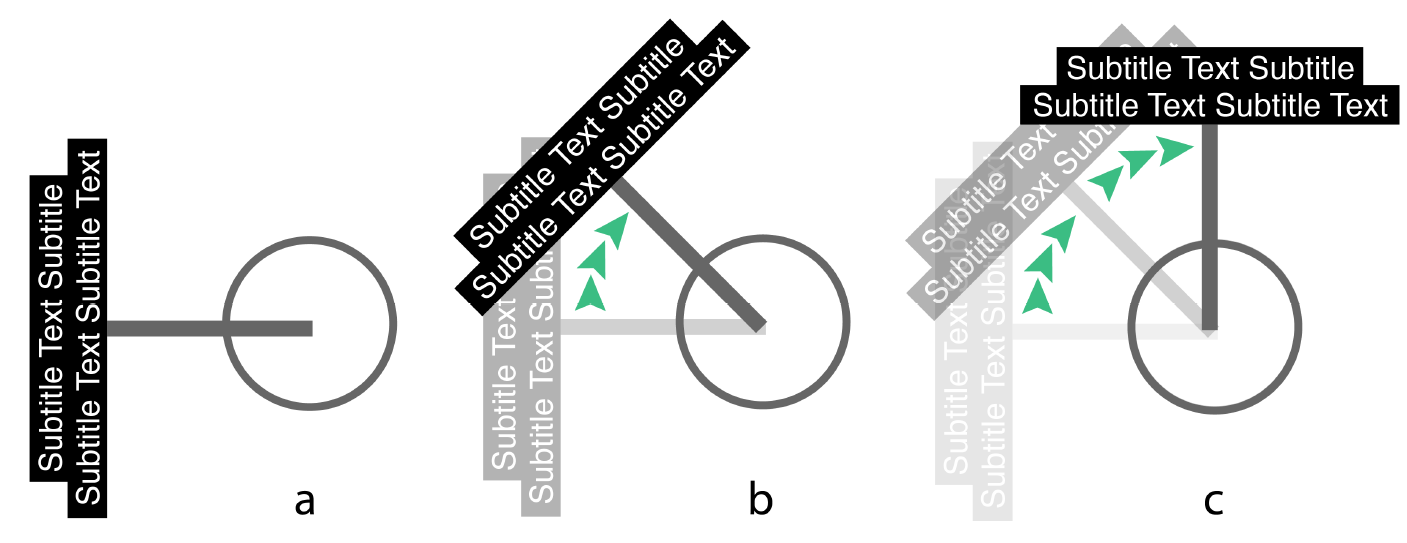
\includegraphics[width=0.8\textwidth]{img/video360/static-follow.png}
    \caption{Static-Follow: The sequence a, b, c demonstrates how as the user turns their head, the subtitles stay fixed to the centre of their field of view. Extracted from \cite{brown_subtitles_2017}.}.
    \label{fig:static_follow}
\end{figure}

When defining the \emph{static-follow} strategy, Brown \emph{et al.} \cite{brown_subtitles_2017} argue that it is a common behavior for showing information in Virtual Reality~(VR) experiences, as part of a ``head-up display'' (HUD). A HUD typically displays graphics that are fixed in front of the viewer at all times regardless of their posture and pose in a VR environment. Figure \ref{fig:static_follow} shows this strategy, which uses the aforementioned HUD mechanic. In this strategy, the subtitles are shown to the viewer as if they were static relative to their head, by following the viewer as they look around the environment. The subtitles are placed 15$^{\circ}$ vertically below eye level. Brown \emph{et al.} \cite{brown_subtitles_2017} mention that a possible caveat of this strategy is that some works have reported that overuse of HUD can cause issues with nausea \cite{laviola2000discussion, sharples2008virtual}.
%%
The work of Meira \emph{et al.} \cite{meira_video_2016} uses this strategy for subtitles positioning. The authors mention that the subtitles are presented at the bottom of the user's viewport and follow their gaze, but they do not mention how many degrees below eye level are used. The work of Matos \emph{et al.} \cite{matos_dynamic_2018} investigates the use of dynamic annotations in 360-degree video, with subtitles being one kind of such annotations. The authors mention the work of Brown \emph{et al.} \cite{brown_subtitles_2017} and call the \emph{static-follow} strategy by \emph{persistent}, in which subtitles~(annotations) are placed in front of the user's view. Rothe \emph{et al.} \cite{rothe_dynamic_2018} refer to this strategy as \emph{static subtitles}, and say that, in a study they conducted, this was the preferred strategy among the ones proposed by \cite{brown_subtitles_2017}. They also mention that the subtitles were positioned at 12.5$^{\circ}$ below eye level. The work of \cite{hughes_disruptive_2019} refers to this strategy as \emph{fixed position in the display picture} and mentions that it is the most common way of using subtitles in 360-degree video. Finally, Montagud \emph{et al.} \cite{montagud_culture_2020} says that there is a follow-up on the work \cite{brown_subtitles_2017} that refers to this strategy as \emph{folow head immediately}. In this follow-up work (a white paper), Brown \emph{et al.} \cite{brown2018exploring} evaluate the four strategies proposed in \cite{brown_subtitles_2017}. 

\begin{figure}[!ht]
    \centering
    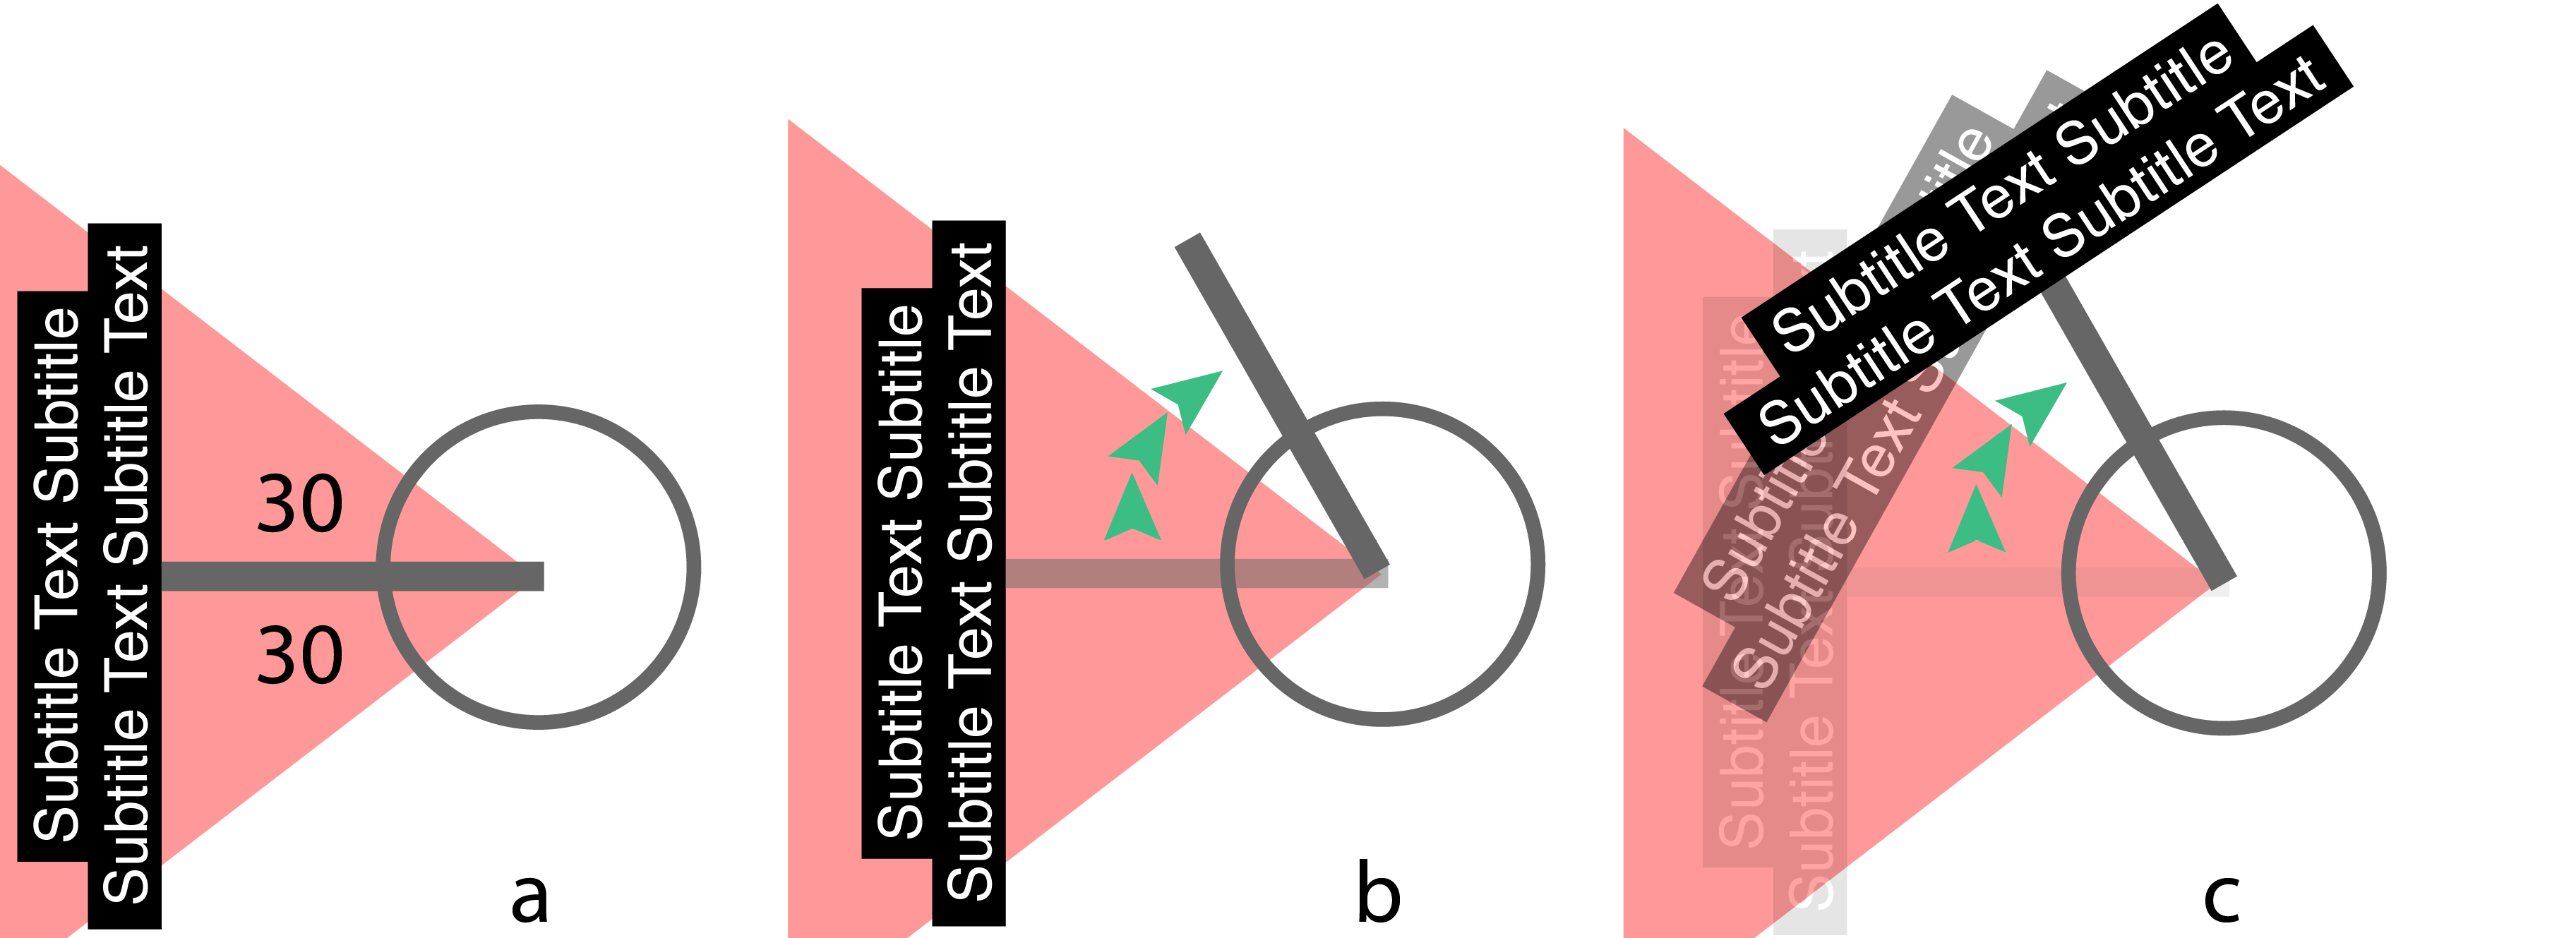
\includegraphics[width=0.8\textwidth]{img/video360/lag-follow.png}
    \caption{Lag-Follow: a. Small user head movements ($<30^{\circ}$) are ignored. b. But turning beyond this boundary c. The subtitles move smoothly to the center of the field-of-view. Extracted from \cite{brown_subtitles_2017}.}
    \label{fig:lag_follow}
\end{figure}

The work of Brown \emph{et al.} \cite{brown_subtitles_2017} defines the \emph{lag-follow}~(see Figure \ref{fig:lag_follow}) strategy to address the sickness related to the \emph{static-follow} strategy while still keeping the subtitles visible to the viewer. Similar to the \emph{static-follow} strategy, the subtitles appear in front of the viewer. It remains in such position~(relative to the environment) until the viewer's head rotates more than the 30$^{\circ}$ threshold. The subtitles then smoothly rotate to be in front of the viewer again. The main objective of this strategy is to provide freedom of movement to the viewer without an immediate reaction from subtitles. However, Brown \emph{et al.} \cite{brown_subtitles_2017} say that this strategy may cause the viewer to reread the subtitles, which is not desirable.
%%
The work of Matos \emph{et al.} \cite{matos_dynamic_2018} describes a strategy that is the same as this one. It is called \emph{floating}, it starts in a position and floats into the viewer's field-of-view. Similar to what was described on the \emph{static-follow} strategy, the work of Montagud \emph{et al.} \cite{montagud_culture_2020} refers to this strategy with a different name (\emph{follow with lag}) but having the same definition.

\subsection{World-Referenced Subtitles}
\label{subsec:world_referenced}

In this category, the subtitles are positioned by taking the 360-degree environment as a reference. 
As referenced in Hughes \emph{et al.} \cite{hughes_disruptive_2019}, this category of strategy leads to better results in comfort~\cite{rothe2018positioning}. Roth \emph{et al.} \cite{rothe2018positioning}, as referenced in Hughes \emph{et al.} \cite{hughes_disruptive_2019}, also say that world-referenced subtitles conflict, in general, with the requirement that a user must always be able to read the subtitle text because it limits the user's freedom of exploring the scene.
We have identified two strategies following this category: \emph{repeated subtitles} and \emph{appear subtitles}. These strategies are described in the following paragraphs. 

\begin{figure}[!ht]
    \centering
    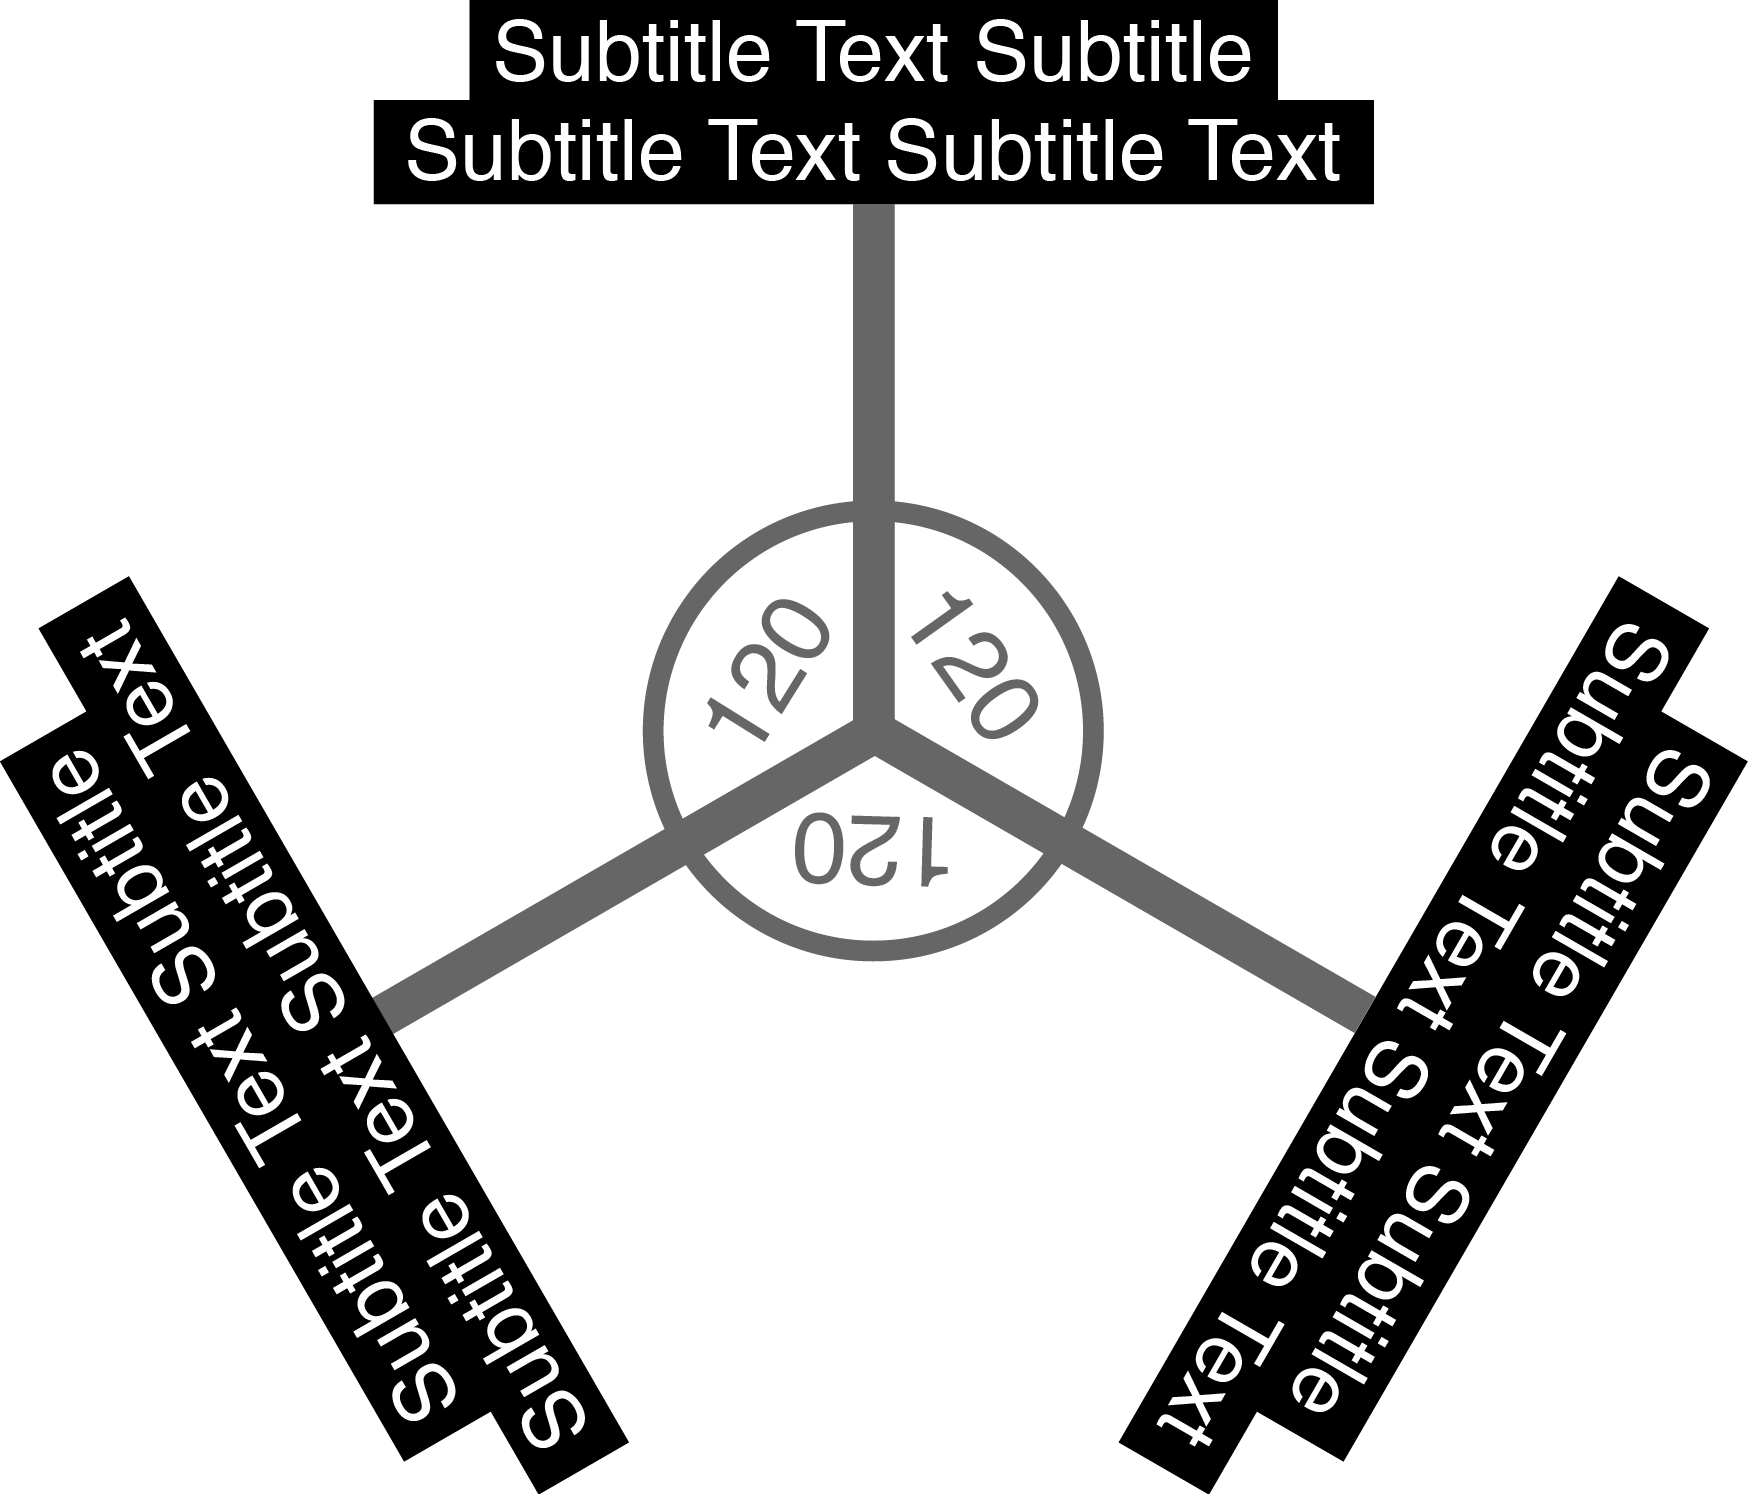
\includegraphics[width=0.4\textwidth]{img/video360/120_subtitles.png}
    \caption{Three repeated subtitles (having the same text) are located in the environment at 120$^{\circ}$ angles around the viewer. Extracted from \cite{brown_subtitles_2017}.}
    \label{fig:120_subtitles}
\end{figure}

In the \emph{repeated subtitles} strategy, the subtitles are placed around the user. These subtitles stay fixed in the environment and do not follow the user's head motion. Figure \ref{fig:120_subtitles} shows three repeated subtitles evenly spaced by angles of 120°. Such figure was extracted from the work of Brown \emph{et al.} \cite{brown_subtitles_2017}. The authors argue that one of the main advantages of this strategy for subtitles positioning is that the subtitles could be ``burnt-in'' to the video using a video editor. This strategy is referenced as \emph{120-degree} in the work of Brown \emph{et al.} \cite{brown_subtitles_2017}, and as \emph{evenly spaced} in the work of Montagud \emph{et al.} \cite{montagud_culture_2020}. A caveat of this strategy, mentioned by Brown \emph{et al.} \cite{brown_subtitles_2017}, is that it may cover important content located in unfortunate positions. 
%%
The work of Li \emph{et al.} \cite{li_impacts_2018} uses this strategy to evaluate the impacts of subtitles in 360-degree video journalism. They do not evaluate the subtitles positioning itself, but the impact of the subtitles. The work of Chen \emph{et al.} \cite{chen_film_2017} uses this strategy for positioning subtitles while investigating film language in society news using 360-degree videos of The New York Times. During their study, some participants found the \emph{repeated subtitles} strategy confusing as they thought, in some moments, that the subtitles in different positions had a different text.


\begin{figure}[!ht]
    \centering
    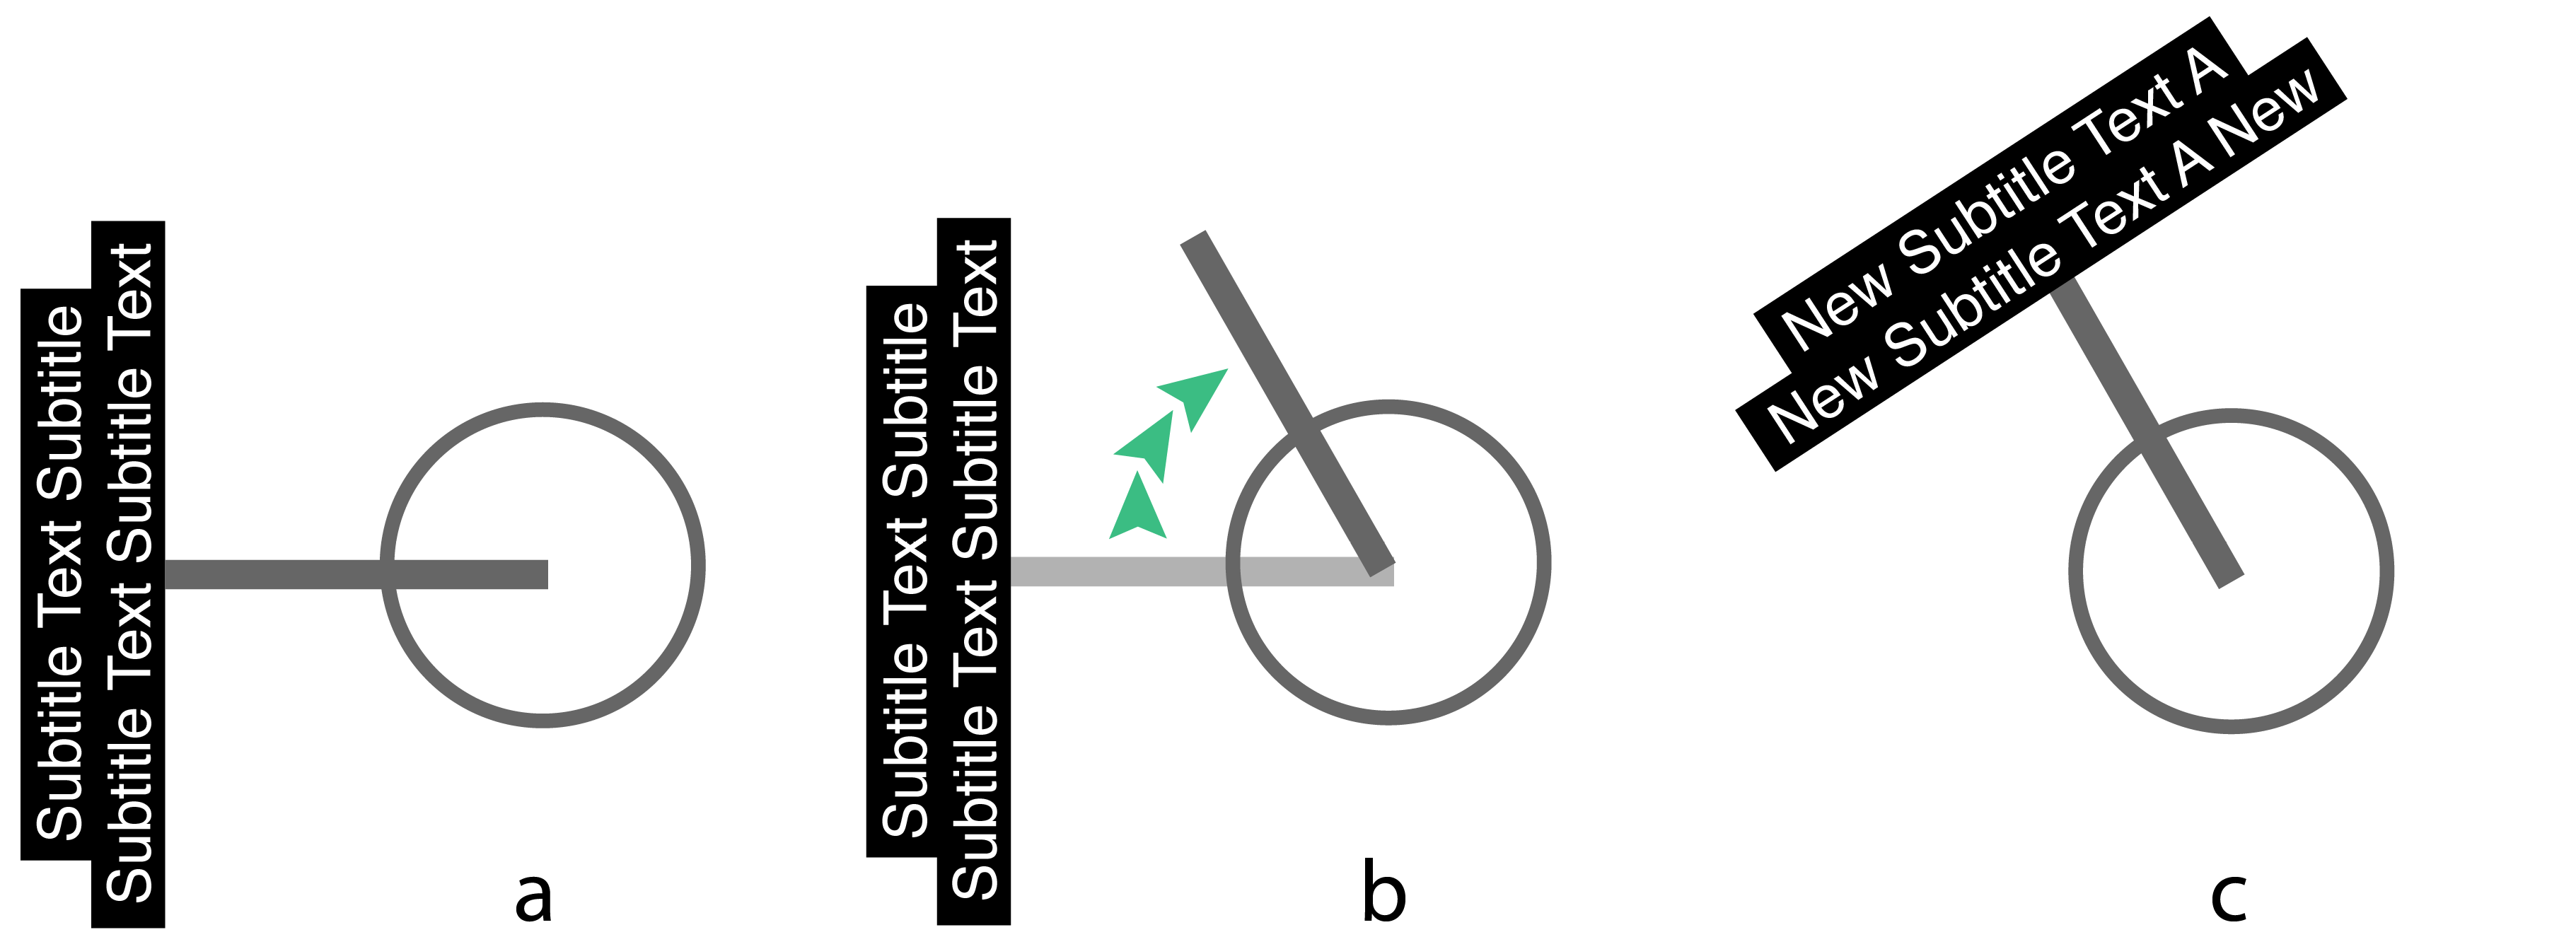
\includegraphics[width=0.8\textwidth]{img/video360/appear.png}
    \caption{Appear: a. A subtitle appears at the centre of the user's view. b. If the user moves before the subtitle is due to change, it will remain static in the environment. c. When a new subtitle is shown, it will appear at the centre of the user's view again. Extracted from \cite{brown_subtitles_2017}.}
    \label{fig:appear_subtitle}
\end{figure}

According to Brown \emph{et al.} \cite{brown_subtitles_2017}, the \emph{appear subtitles} strategy was designed based on feedback from a user who was hard of hearing, they had the idea of creating a strategy in which the viewer can dismiss the subtitle after reading it. As it is depicted in Figure \ref{fig:appear_subtitle}, the subtitles are placed at the center of the user's field of view horizontally, 15$^{\circ}$ below eye level. If the viewer moves their head, the subtitles remain static within the environment and do not follow their gaze. This strategy is also referenced as \emph{appear in front, then fixed} in the work of Montagud \emph{et al.} \cite{montagud_culture_2020}. A possible caveat of this strategy, mentioned by Brown \emph{et al.} \cite{brown_subtitles_2017}, is that the subtitles may be positioned in spurious locations if the viewer is quickly moving their head.

\subsection{Dynamic Subtitles}
\label{subsection:dynamic_subtitles}

In this category, the position of subtitles dynamically changes and depends on the scene \cite{rothe_dynamic_2018}. As referring to annotations~(that could be subtitles), Matos \emph{et al.} \cite{matos_dynamic_2018} say that there are cases where the point of interest is moving through the video, which requires a dynamic annotation that follows its movement. One strategy that we have identified in this category is the \emph{speaker-following subtitles} strategy.

In the \emph{speaker-following subtitles} strategy, the subtitles are placed close to the speaker~(see Figure \ref{fig:speaker_following}). Since the speakers may move during the video, this strategy fits in the \emph{dynamic subtitles} category. This strategy also helps in the issue of \emph{speaker identification}, as all persons in the room are visible in a 360-degree video~\cite{rothe_dynamic_2018}.  
%%
Rothe \emph{et al.} \cite{rothe_dynamic_2018} compared \emph{speaker-following} subtitles with the \emph{static-follow} strategy regarding task workload, simulator sickness and presence. For evaluating each of these dimensions, the authors used, respectively, the following questionnaires: NASA-TLX~\cite{nasa_hart1988development}; Simulator Sickness Questionaire~\cite{sickness_kennedy1993simulator}; and Presence Questionaire~\cite{presence_witmer1998measuring}. When asking which strategy the participants preferred, the authors received balanced answers. However, \emph{speaker-following} subtitles led to a higher score of presence, less sickness, and lower workload~\cite{rothe_dynamic_2018}.

\begin{figure}[!ht]
    \centering
    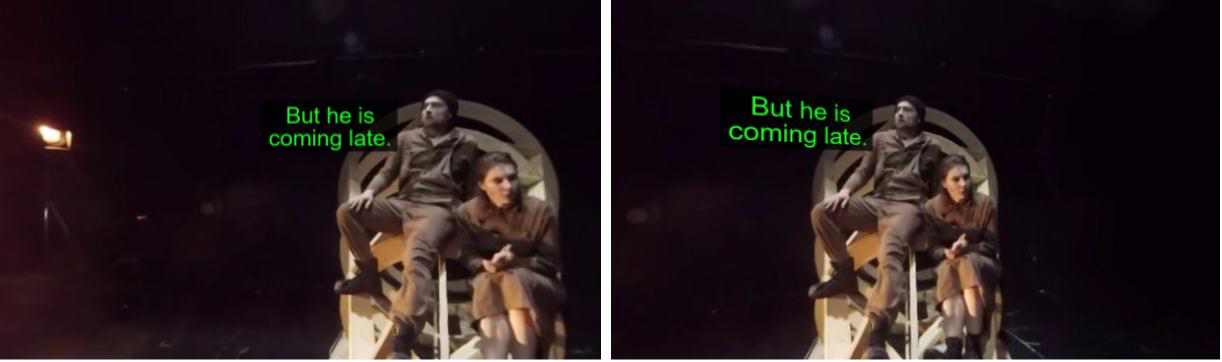
\includegraphics[width=0.95\textwidth]{img/video360/speaker-following.png}
    \caption{Speaker-following subtitles. Extracted from \cite{hughes_disruptive_2019}.}
    \label{fig:speaker_following}
\end{figure}

Similar to the work of Rothe \emph{et al.} \cite{rothe_dynamic_2018}, we intend to position subtitles close to the speakers in the 360-video. The main difference of our work, however, is that we automatically detect the actors present in a 360-video and use their position for placing the subtitles according to an authoring model we propose. In our authoring model, we can also determine the direction that the user is looking at. We use that to position the subtitles as \emph{static-follow} when the actor speaking is not visible to the user. In this way, the disadvantage of \emph{speaker-following} subtitles being not always visible is suppressed.